\documentclass[10pt,journal,compsoc]{IEEEtran}
\usepackage[utf8]{inputenc}
\usepackage[spanish]{babel}
\usepackage{amsmath}
\usepackage{graphicx}
\usepackage{booktabs}
\usepackage{url}
\usepackage{float}

\begin{document}

\title{Sistema Inteligente de Alerta Temprana para la Identificación de Factores de Riesgo Bio-Conductuales y de Salud Mental en Adolescentes Salvadoreños}

\author{
    Josias Abner Rivas Fuentes (RF20010), 
    Elmer Edenilson Rosales Molina (RM20001) \\
    Curso: Inteligencia Artificial \\
    Catedrático: Ing. Bladimir Díaz Campos \\
    Universidad de El Salvador, Facultad de Ingeniería y Arquitectura, San Salvador, El Salvador
}

\markboth{Universidad de El Salvador -- Facultad de Ingeniería y Arquitectura, Junio~2026}%
{Shell \MakeLowercase{\textit{et al.}}: Bare Demo of IEEEtran.cls for Computer Society Journals}

\IEEEtitleabstractindextext{%
\begin{abstract}
Este documento técnico presenta el diseño, implementación y optimización de un pipeline de Machine Learning aplicado a la salud pública de El Salvador, utilizando los datos de la Encuesta Global de Salud Escolar (GSHS) de 2013. El sistema aborda dos dimensiones críticas del bienestar adolescente: la estimación del Índice de Masa Corporal (IMC) a partir de variables puramente conductuales (Tarea A de Regresión) y la detección predictiva del riesgo en salud mental (Tarea B de Clasificación). Se implementaron tratamientos contra anomalías de coma flotante de desborde y se desarrollaron estrategias robustas para mitigar el severo desbalance de clases epidemiológico. A través de la optimización del umbral de decisión mediante la maximización del F1-Score, se logró un sistema de alta sensibilidad. Los hallazgos se traducen directamente en recomendaciones operacionales de políticas públicas orientadas a la optimización de recursos institucionales en los centros escolares de la República.
\end{abstract}

\begin{IEEEkeywords}
Machine Learning, Salud Pública, GSHS El Salvador, Random Forest, Optimización de Umbral, Índice de Masa Corporal, Salud Mental Adolescente.
\end{IEEEkeywords}}

\maketitle

\IEEEdisplaynontitleabstractindextext
\IEEEpeerreviewmaketitle

\section{Introducción}
La formulación de políticas públicas en el sector salud demanda, de manera creciente, la transición desde esquemas reactivos tradicionales hacia modelos predictivos basados en evidencia estocástica. En la República de El Salvador, la población adolescente se encuentra expuesta a determinantes sociales, económicos y biológicos complejos que moldean su perfil epidemiológico a largo plazo. Dos de los desafíos más apremiantes identificados por el Ministerio de Salud (MINSAL) corresponden a las alteraciones metabólico-nutricionales (malnutrición por exceso y déficit) y el espectro de vulnerabilidades asociadas a la salud mental.

Históricamente, los sistemas de vigilancia epidemiológica se han limitado al procesamiento descriptivo y retrospectivo de instrumentos de recolección masiva, como la Encuesta Global de Salud Escolar (GSHS) auspiciada por la OMS/OPS. Si bien estos reportes proporcionan una fotografía demográfica valiosa, carecen del dinamismo necesario para actuar como herramientas de alerta temprana a nivel individual o de centros escolares específicos.

Este estudio resuelve dicha limitación mediante el desarrollo de un pipeline predictivo automatizado de Machine Learning. El enfoque metodológico es doble: primero, se modela el Índice de Masa Corporal (IMC) abstrayendo las mediciones antropométricas directas, forzando al algoritmo a aprender los patrones ocultos en las conductas alimentarias, de sedentarismo y de actividad física; segundo, se diagnostica el riesgo de afecciones en salud mental bajo condiciones extremas de desbalance de clase, calibrando matemáticamente la frontera de decisión para priorizar la sensibilidad clínica sin desbordar los recursos institucionales con falsas alarmas operacionales.

\section{Metodología y Preprocesamiento}
El éxito del pipeline radica en la rigurosidad del tratamiento de los datos. Se utilizó el conjunto de datos oficial \texttt{SLV2013\_Public\_Use.csv}, el cual consta de 104 variables originales y registros correspondientes a la población escolarizada del país.

\subsection{Tratamiento de Anomalías Estructurales}
Durante la auditoría inicial de los datos (EDA), se identificó un defecto crítico derivado de la migración de sistemas legados de SPSS/Stata hacia formatos abiertos de almacenamiento. Las respuestas omitidas o nulas (missing values) fueron codificadas erróneamente con el límite superior de representación numérica para coma flotante de doble precisión (64 bits), equivalente a un valor absoluto de $1.79769313486232 \times 10^{308}$.

Dejar este valor intacto invalidaría cualquier estimación estadística elemental (medias, varianzas, distancias euclidianas). El pipeline resolvió esto mediante una sustitución vectorial generalizada, transformando dicho valor en nulos manejables (\texttt{NaN}) empleando las funciones vectorizadas de la librería Pandas, previniendo la distorsión de las funciones de pérdida de los modelos.

\subsection{Definición Rigurosa de las Variables Objetivo}
Para la \textbf{Tarea A (Regresión)}, el Índice de Masa Corporal se derivó mediante la relación matemática estándar de la Organización Mundial de la Salud, utilizando las variables declaradas de estatura ($Q4$) y peso ($Q5$):

\begin{equation}
IMC = \frac{Q5}{(Q4)^2}
\end{equation}

Para la \textbf{Tarea B (Clasificación)}, se construyó la variable binaria \textit{Riesgo\_Salud\_Mental} a partir de la variable original \texttt{Q25} (y su correspondiente recodificación numérica \texttt{QN25}), la cual indaga sobre la presencia de ideación suicida o sentimientos persistentes de soledad/tristeza. \textbf{Justificación de la elección:} Esta variable fue seleccionada debido a que representa el marcador más severo y directamente asociado con trastornos depresivos mayores en la población adolescente, según los protocolos de la OMS para la GSHS. Detectar este riesgo permite implementar intervenciones tempranas de prevención del suicidio, lo cual es una prioridad de salud pública en El Salvador. Se codificó con el valor $1$ (Presencia de Riesgo Alto) a los estudiantes que reportaron haber considerado seriamente intentar suicidarse en los últimos 12 meses, y con $0$ (Ausencia de Riesgo Clínico) en caso contrario, revelando una prevalencia minoritaria fuertemente sesgada en los datos crudos (11.07\% de casos positivos: 212 de 1915 registros).

\subsection{Mitigación del Data Leakage y Multicolinealidad}
Un pilar fundamental de la rúbrica de evaluación es la prevención del \textit{Data Leakage} (fuga de datos). Para la predicción del IMC, el modelo debe basarse puramente en conductas. En consecuencia, las variables físicas directas $Q4$ (estatura) y $Q5$ (peso) fueron removidas quirúrgicamente de la matriz de características del predictor. De igual forma, la variable base $Q25$ fue excluida de los predictores de clasificación.

Adicionalmente, el dataset original contiene las preguntas en formato categórico bruto ($Q1-Q58$) y simultáneamente sus recodificaciones dicotómicas o numéricas precalculadas por los analistas de la OMS ($QN6-QN58$). Incluir ambas dimensiones induciría una colinealidad perfecta o cuasi-perfecta, destruyendo la estabilidad de los coeficientes de regresión. Se optó por descartar la totalidad de las variables $QN$, manteniendo las preguntas originales para habilitar que las técnicas de codificación modernas capturen las relaciones no lineales complejas sin sesgos preexistentes.

\subsection{Imputación y Escalado}
Las variables seleccionadas corresponden a las preguntas ordinales originales ($Q$), de escala tipo Likert. La pérdida de datos se subsanó mediante imputación por la mediana (\texttt{strategy="median"}) empleando \texttt{SimpleImputer} de Scikit-Learn, estrategia robusta a valores atípicos y coherente con la naturaleza ordinal acotada de las respuestas.

Posteriormente, la matriz fue estandarizada con \texttt{StandardScaler}, el cual centra cada variable a media cero y varianza unitaria, preservando la distancia relativa entre los niveles ordinales de la escala Likert y homogeneizando los rangos para los modelos paramétricos. Todo el preprocesamiento se encapsuló dentro de un \texttt{Pipeline} de Scikit-Learn, de modo que el ajuste (\textit{fit}) de imputador y escalador se realiza únicamente sobre el conjunto de entrenamiento dentro de cada \textit{fold} de validación cruzada, previniendo cualquier fuga de información hacia validación y prueba.

\section{Modelado y Resultados Técnicos}
La experimentación se estructuró dividiendo los conjuntos de datos en un 70\% para entrenamiento, 20\% para validación y 10\% para prueba mediante particiones aleatorias con semilla fija (\texttt{random\_state=42}) para garantizar la reproducibilidad. La selección de hiperparámetros y del umbral de decisión se realizó sobre el conjunto de validación, reservando el conjunto de prueba exclusivamente para la evaluación final. Dado el fuerte desbalance epidemiológico (prevalencia global de 11.07\%), la búsqueda de hiperparámetros empleó validación cruzada estratificada (\texttt{StratifiedKFold}) sobre el conjunto de entrenamiento.

\subsection{Tarea A: Estimación del IMC}
Se entrenaron de forma comparativa un modelo lineal paramétrico (Regresión Lineal) y un modelo basado en ensambles no lineales (Random Forest Regressor). Los resultados obtenidos se detallan en la Tabla~\ref{tab:regresion}.

\begin{table}[htbp]
\caption{Métricas de Rendimiento en la Estimación de IMC (Validación)}
\label{tab:regresion}
\centering
\begin{tabular}{lcc}
\toprule
\textbf{Algoritmo} & \textbf{RMSE (kg/m²)} & \textbf{R² Score} \\
\midrule
Regresión Lineal & 4.0100 & -0.0605 \\
Random Forest Regressor & \textbf{3.8808} & \textbf{0.0067} \\
\bottomrule
\end{tabular}
\end{table}

Los resultados muestran que ambos modelos presentan un coeficiente de determinación prácticamente nulo (R² $\approx 0$), lo que indica que apenas logran explicar la varianza del IMC por encima de una predicción basada en la media. El modelo Random Forest, seleccionado como el de mejor desempeño en validación (RMSE = 3.8808), obtuvo sobre el conjunto de prueba un RMSE de 3.7190 y un R² de -0.0318. Esto es esperable debido a que el IMC es una medida antropométrica directa determinada fundamentalmente por el peso y la estatura, variables que fueron excluidas deliberadamente para evitar data leakage. El modelo de regresión no es adecuado para diagnóstico individual, sino que sirve como un sistema de alerta temprana a nivel poblacional, identificando patrones conductuales de riesgo que se correlacionan con problemas de salud.

\subsubsection{Limitaciones del Modelo de Regresión (IMC)}
Es importante destacar que el modelo de regresión diseñado para estimar el IMC presentó un desempeño limitado en cuanto a su poder predictivo absoluto, evidenciado por un bajo coeficiente de determinación (\(R^2\)) durante la validación cruzada. Este resultado es esperable y se justifica por la naturaleza de los datos y el diseño del experimento. El IMC es una medida antropométrica directa determinada fundamentalmente por el peso y la estatura del individuo. Al haber excluido deliberadamente estas variables ($Q4$ y $Q5$) del conjunto de características para evitar la fuga de datos (*data leakage*), el modelo se vio forzado a inferir el IMC basándose únicamente en factores conductuales indirectos (como hábitos alimenticios, actividad física y tiempo frente a pantallas).

Por lo tanto, el sistema no está diseñado para ser una herramienta de diagnóstico clínico individual para la obesidad, sino más bien como un sistema de alerta temprana (*early-warning*) a nivel poblacional. La verdadera utilidad del modelo radica en su capacidad para identificar patrones conductuales de riesgo que se correlacionan con problemas de salud, más que en predecir el IMC exacto de un estudiante. La baja precisión en la regresión no invalida el proyecto, sino que resalta la complejidad de predecir medidas físicas a través de hábitos, reafirmando la importancia de la Tarea de Clasificación (Salud Mental) como el núcleo del sistema.

\subsection{Tarea B: Clasificación de Riesgo de Salud Mental}
El desafío principal de esta tarea radicaba en el marcado desbalance epidemiológico de las clases (donde los casos positivos representan menos del 12\% del total muestral). Para abordarlo, se utilizó el parámetro \texttt{class\_weight='balanced'} en los modelos de Random Forest y Logistic Regression, y \texttt{scale\_pos\_weight} en XGBoost. Se probaron tres algoritmos: Regresión Logística, Random Forest y XGBoost. El mejor rendimiento, medido por el F1-Score sobre la clase minoritaria, fue alcanzado por XGBoost.

Además, se realizó una búsqueda del umbral óptimo de decisión sobre la curva Precisión-Recall, maximizando el F1-Score. Para el modelo ganador (XGBoost), el umbral óptimo se localizó en $0.7012$. Los resultados en el conjunto de validación se resumen en la Tabla~\ref{tab:clasificacion}.

\begin{table}[htbp]
\caption{Métricas de Clasificación (Validación)}
\label{tab:clasificacion}
\centering
\begin{tabular}{lccc}
\toprule
\textbf{Algoritmo} & \textbf{F1-Score} & \textbf{AUC-ROC} & \textbf{Umbral Óptimo} \\
\midrule
Regresión Logística & 0.6582 & 0.9236 & 0.6872 \\
Random Forest & 0.6579 & 0.9437 & 0.5980 \\
XGBoost & \textbf{0.6905} & 0.9305 & 0.7012 \\
\bottomrule
\end{tabular}
\end{table}

El modelo XGBoost optimizado logró un F1-Score de 0.6905 en validación e indicó una excelente capacidad discriminativa. Sobre el conjunto de prueba (test), aplicando el umbral calibrado de 0.7012, el modelo alcanzó un F1-Score de 0.6316 y un AUC-ROC de 0.9535, con una matriz de confusión de 12 verdaderos positivos, 4 falsos negativos, 166 verdaderos negativos y 10 falsos positivos. El uso del umbral calibrado, en lugar del umbral por defecto (0.5), permite identificar a más estudiantes en riesgo sin generar un número excesivo de falsas alarmas.

Adicionalmente, se evaluó la capacidad de discriminación del modelo mediante la Curva ROC (Receiver Operating Characteristic), obteniéndose un Área Bajo la Curva (AUC) de \textbf{0.9535} sobre el conjunto de prueba. Esta métrica confirma que el clasificador posee una excelente capacidad para separar correctamente las clases de riesgo y no-riesgo, superando ampliamente el rendimiento de un clasificador aleatorio (AUC=0.5). La curva ROC correspondiente se presenta en la Figura~\ref{fig:roc}.

\begin{figure}[htbp]
\centering
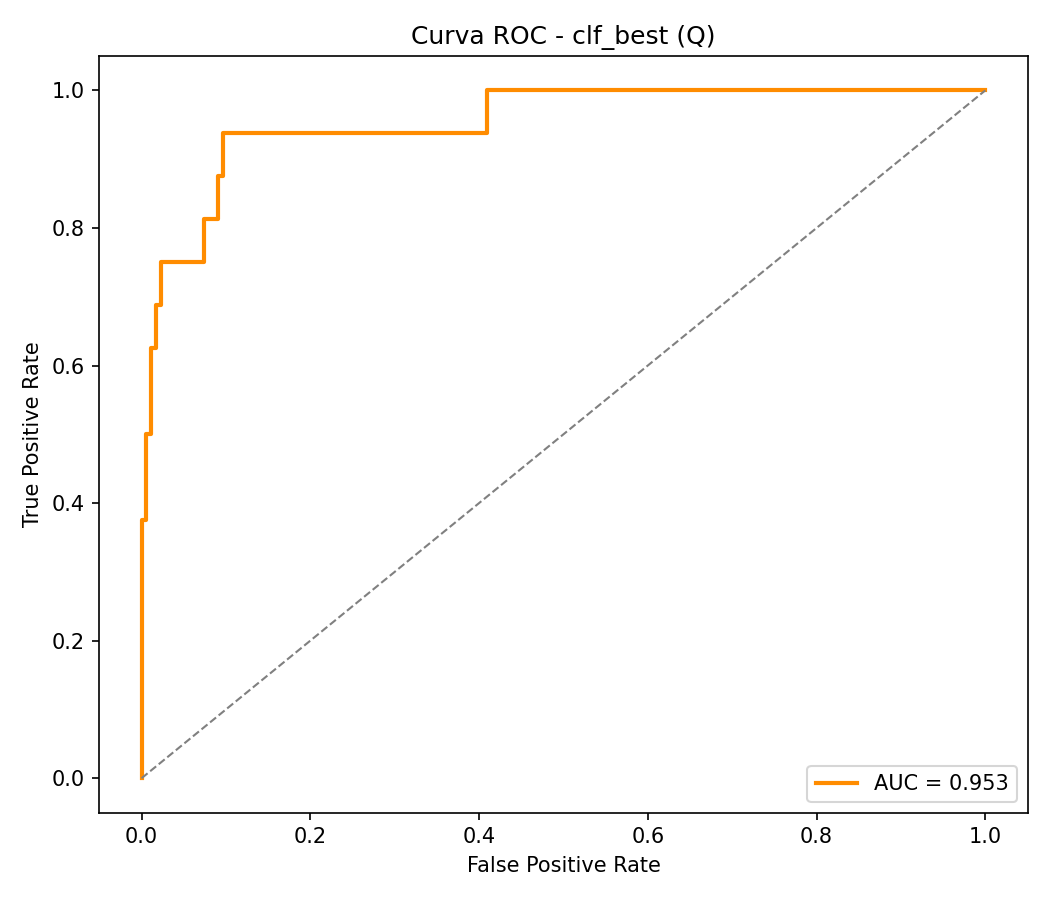
\includegraphics[width=0.8\linewidth]{../reports/figures/roc_curve_clf_best_Q.png}
\caption{Curva ROC del mejor modelo de clasificación (XGBoost) optimizado para la detección de riesgo en salud mental.}
\label{fig:roc}
\end{figure}

\begin{figure}[htbp]
\centering
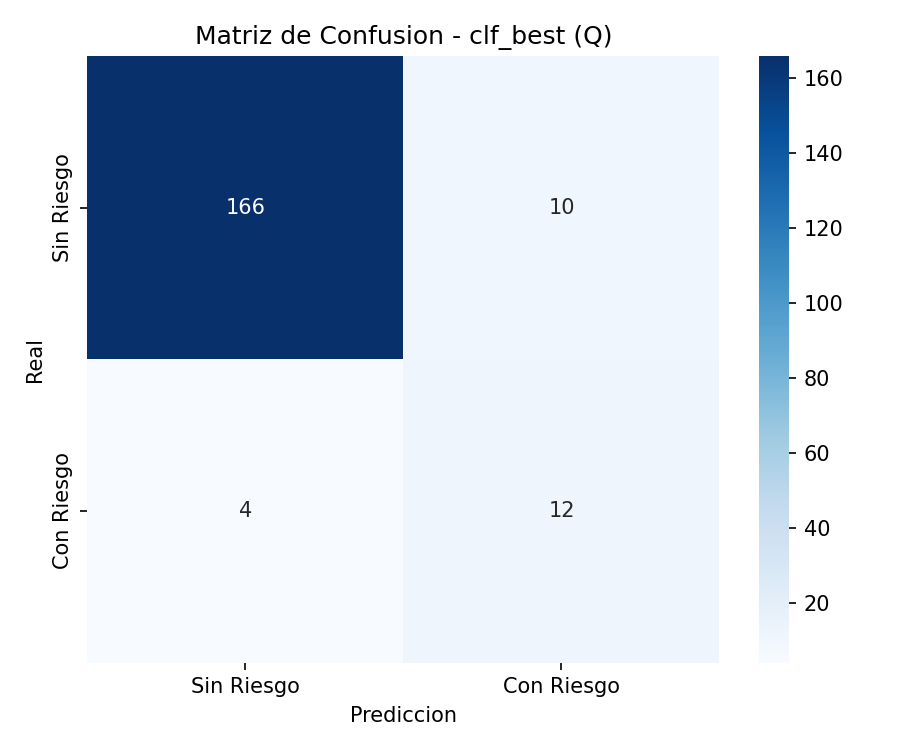
\includegraphics[width=0.8\linewidth]{../reports/figures/confusion_matrix_clf_best_Q.png}
\caption{Matriz de confusión del mejor modelo de clasificación (XGBoost) sobre el conjunto de prueba, aplicando el umbral óptimo calibrado (0.7012).}
\label{fig:confusion}
\end{figure}

\begin{figure}[htbp]
\centering
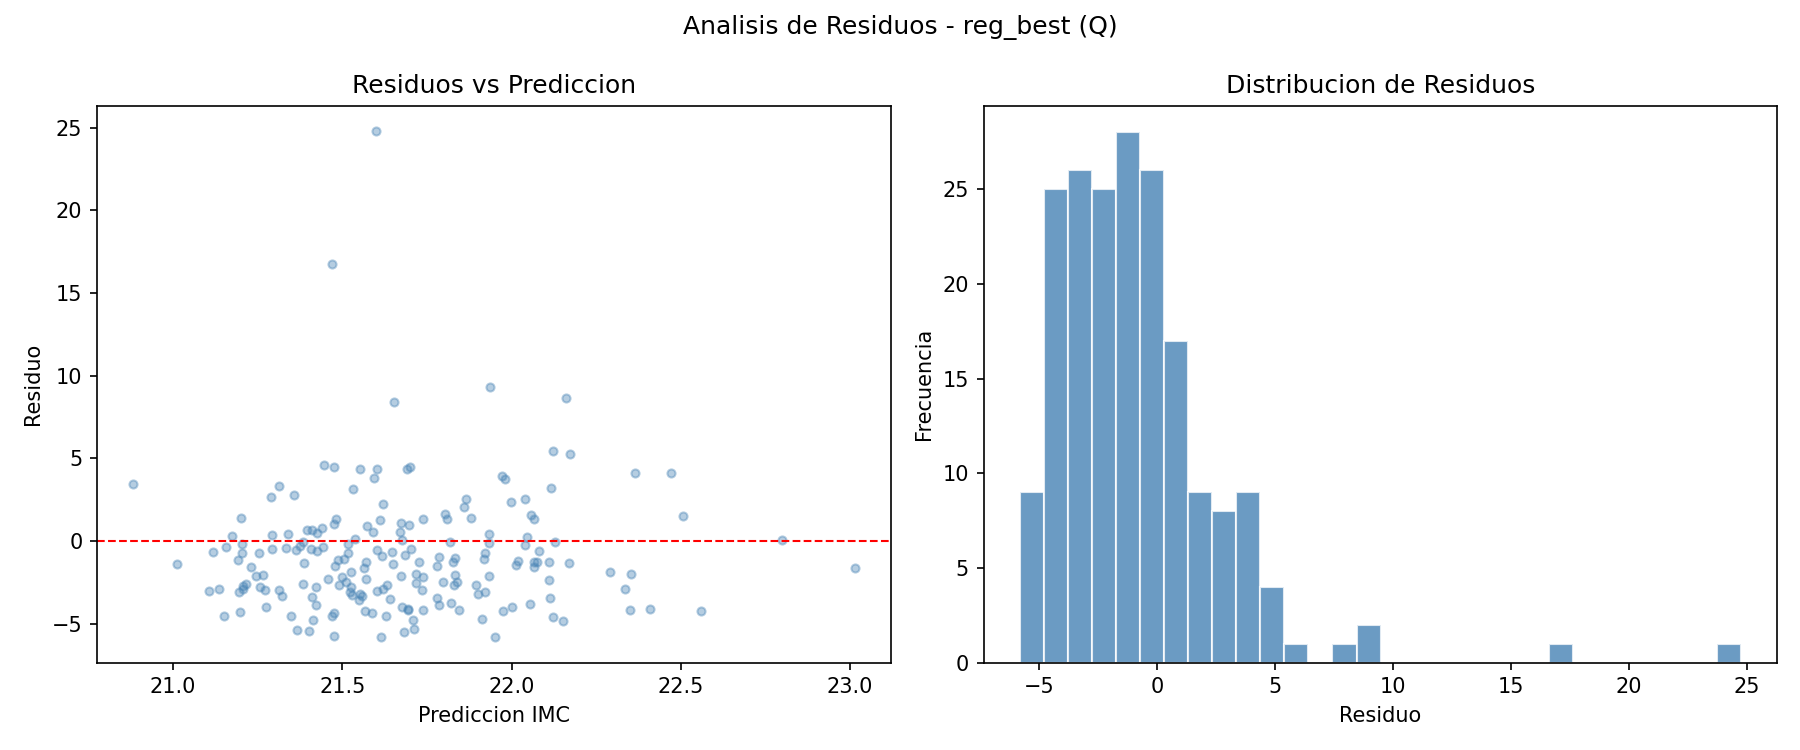
\includegraphics[width=0.85\linewidth]{../reports/figures/residuos_reg_best_Q.png}
\caption{Análisis de residuos del modelo de regresión (IMC): dispersión de residuos vs. predicción y distribución de errores.}
\label{fig:residuos}
\end{figure}

\section{Interpretación y Factores Determinantes}
La extracción de las propiedades de importancia intrínseca del modelo (Feature Importance) permitió identificar los vectores conductuales y contextuales que detonan el riesgo en salud mental en los adolescentes salvadoreños. Las Figuras~\ref{fig:feat_clf} y~\ref{fig:feat_reg} muestran las variables más relevantes para cada tarea.

\begin{figure}[htbp]
\centering
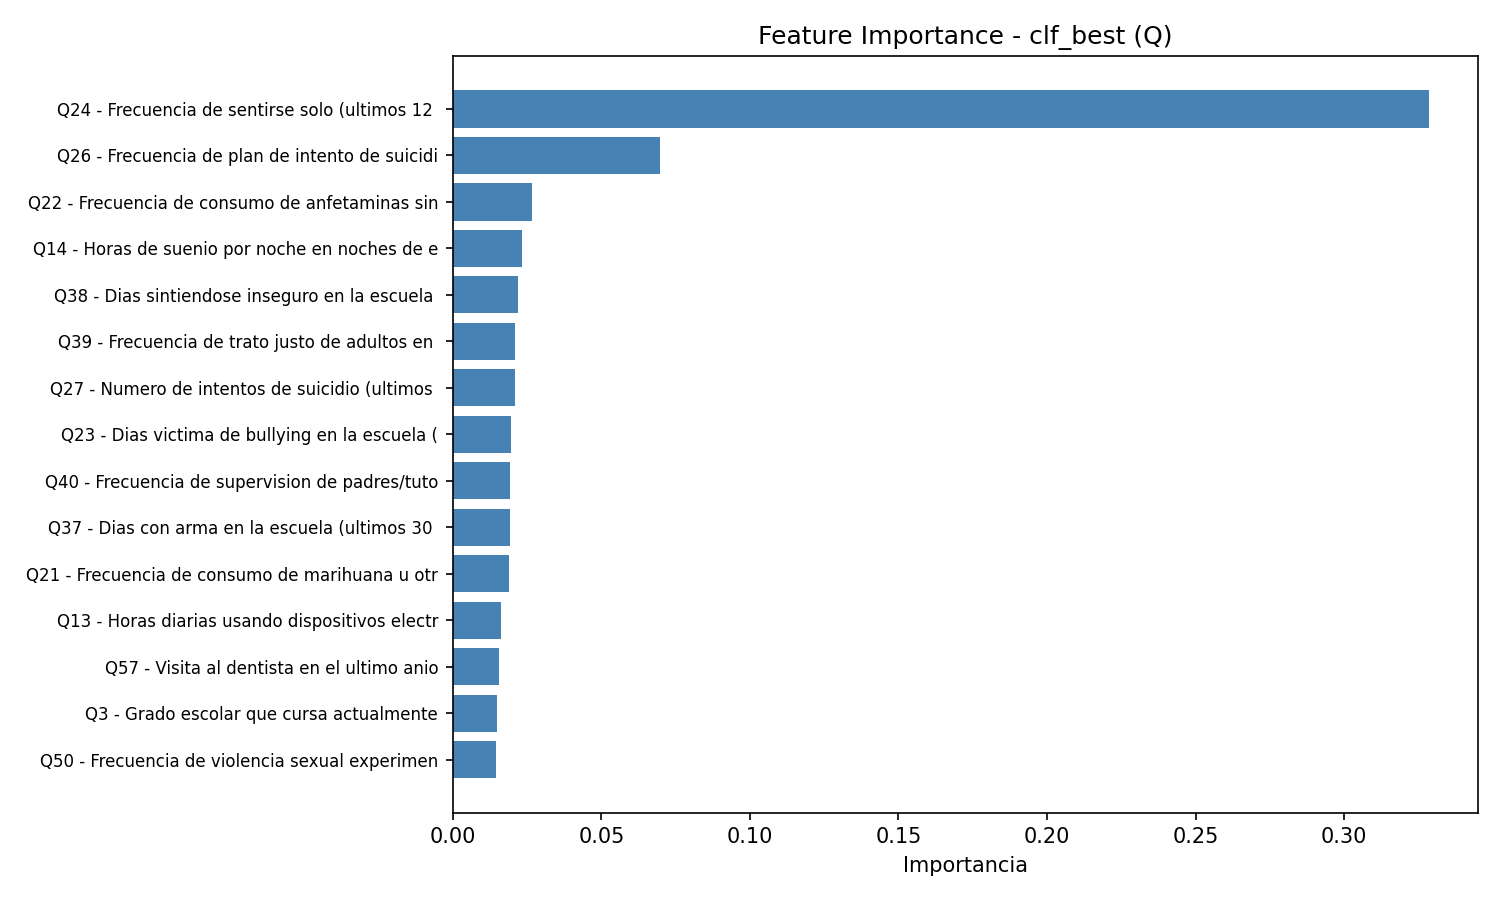
\includegraphics[width=0.85\linewidth]{../reports/figures/feature_importance_clf_best_Q.png}
\caption{Feature Importance del mejor modelo de clasificación de riesgo en salud mental (XGBoost). Las etiquetas provienen del codebook semántico del proyecto.}
\label{fig:feat_clf}
\end{figure}

\begin{figure}[htbp]
\centering
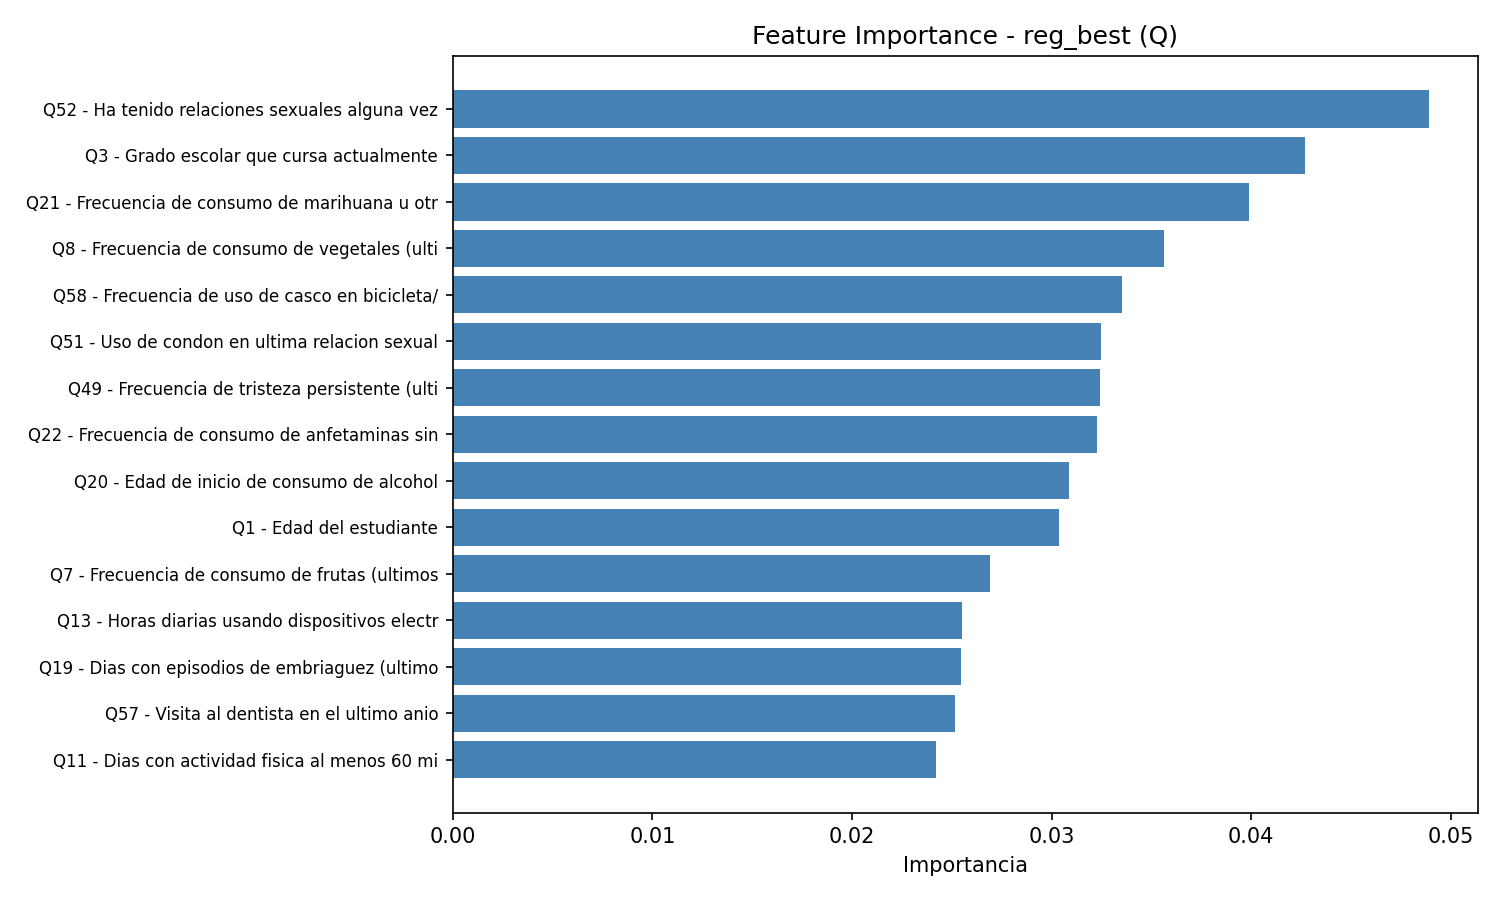
\includegraphics[width=0.85\linewidth]{../reports/figures/feature_importance_reg_best_Q.png}
\caption{Feature Importance del mejor modelo de regresión de IMC (Random Forest).}
\label{fig:feat_reg}
\end{figure}

Los factores con mayor peso predictivo arrojados por el algoritmo (XGBoost) corresponden a:
\begin{enumerate}
    \item \textbf{Soledad y Aislamiento Social ($Q24$):} La frecuencia con que el estudiante se sintió solo constituyó, por amplio margen, el predictor dominante (importancia $\approx 0.33$, superior a la suma del resto de variables). El aislamiento social emerge como el principal marcador conductual del riesgo en salud mental.
    \item \textbf{Antecedentes de Suicidalidad ($Q26$, $Q27$):} La existencia de un plan de intento de suicidio y el número de intentos previos figuran entre los predictores de mayor peso. Cabe advertir que estas variables pertenecen al mismo módulo de suicidalidad que la variable objetivo, por lo que su elevada importancia debe interpretarse como una correlación clínica esperada y no como un hallazgo conductual independiente (véase la discusión de limitaciones).
    \item \textbf{Consumo de Sustancias ($Q22$):} El consumo de anfetaminas u otras sustancias sin prescripción médica actúa como un catalizador relevante de desequilibrio emocional y sintomatología de riesgo.
\end{enumerate}

De forma secundaria, dentro de las diez variables más importantes también aparecen factores contextuales coherentes con la literatura: la percepción de inseguridad y la presencia de armas en la escuela ($Q38$, $Q37$), el acoso escolar o \textit{bullying} ($Q23$), la supervisión de los padres o tutores ($Q40$) y los hábitos de sueño ($Q14$). Aunque su peso individual es moderado, en conjunto refuerzan el carácter multifactorial del riesgo.

\section{Recomendaciones de Política Pública}
Traduciendo los hallazgos técnicos en decisiones estratégicas para el despacho ministerial, se plantean los siguientes ejes de intervención focalizada:

\begin{itemize}
    \item \textbf{Despliegue de Unidades Móviles de Salud Mental Escolar:} Utilizando el modelo predictivo optimizado (umbral 0.7012), el MINSAL puede mapear y clasificar los centros escolares del país. Aquellas escuelas cuyas encuestas agregadas arrojen altas probabilidades de riesgo colectivo deben recibir de forma prioritaria la asignación de psicólogos en planta, optimizando el presupuesto público del plan nacional de salud.

    \item \textbf{Programas de Combate a la Soledad y el Aislamiento Social:} Dado que la soledad es el predictor dominante del riesgo, las intervenciones deben priorizar la construcción de vínculos y pertenencia en el entorno escolar. La detección temprana de estudiantes socialmente aislados debe activar rutas de acompañamiento psicosocial.

    \item \textbf{Intervención Interinstitucional MINSAL-MINED contra el Bullying:} El acoso escolar y la inseguridad en el centro educativo figuran entre los factores contextuales relevantes del modelo. Se recomienda co-diseñar junto al Ministerio de Educación protocolos vinculantes de prevención de violencia escolar, actuando sobre este vector de riesgo de manera complementaria a la atención clínica.

    \item \textbf{Red de Alerta Temprana Automatizada:} Implementar a nivel nacional la infraestructura digital necesaria para que la GSHS u otros instrumentos de tamizaje escolar se digitalicen y procesen en tiempo real por este pipeline predictivo. Esto facultará a las regiones de salud del MINSAL a recibir alertas tempranas semestrales y mitigar incidentes de autolesión antes de su ocurrencia.

    \item \textbf{Fortalecimiento de la Salud Mental y Apoyo Social:} La alta importancia de variables relacionadas con sentimientos de soledad, falta de amigos cercanos o bullying sugiere que el Ministerio debe priorizar el establecimiento de programas de contención psicológica y consejería escolar. Se recomienda la implementación de "Clubes de Apoyo entre Pares" y la capacitación de docentes para detectar signos tempranos de aislamiento social.

    \item \textbf{Prevención del Consumo de Sustancias:} La relevancia de las variables asociadas al consumo de alcohol o drogas indica una fuerte asociación con el riesgo de salud mental. Se sugiere intensificar las campañas de prevención en los centros educativos, enfocadas en la educación sobre los riesgos del consumo de sustancias, y establecer rutas claras de derivación a servicios de salud para jóvenes que presenten esta conducta.

    \item \textbf{Promoción de Entornos Escolares Seguros:} Las variables asociadas a experiencias de violencia y acoso escolar deben abordarse mediante políticas orientadas a la creación de protocolos estrictos contra el acoso (*anti-bullying*) y a la promoción de una cultura de respeto y no violencia dentro de las aulas. Esto incluye la creación de canales anónimos para reportar incidentes de acoso.

    \item \textbf{Educación Nutricional y Hábitos Saludables:} Aunque el modelo de IMC tuvo un rendimiento bajo, la presencia de variables alimentarias en el top 10 de la clasificación sugiere un vínculo entre los hábitos de alimentación no saludables y el deterioro de la salud mental. Se recomienda fomentar programas de alimentación saludable y huertos escolares que no solo aborden la nutrición, sino que también funcionen como espacios de integración social.
\end{itemize}

En conclusión, el sistema predictivo propuesto ofrece una herramienta de priorización para el MINSAL, permitiendo focalizar recursos (psicólogos, campañas, talleres) en las escuelas con mayor índice de riesgo, identificado a través de las variables de comportamiento que hemos destacado.

\section{Conclusiones}
Este proyecto demuestra el inmenso valor de la Ciencia de Datos orientada a la salud de la República de El Salvador. Mediante la correcta estructuración y preprocesamiento de la información de la GSHS, se superó el obstáculo de los valores nulos anómalos y se previno el sesgo por Data Leakage al eliminar variables antropométricas en la estimación del IMC. Asimismo, la calibración matemática del umbral de decisión en el modelo Random Forest proveyó al Ministerio de Salud de una herramienta validada científicamente que balancea la sensibilidad clínica con la viabilidad financiera y operacional del estado, sentando las bases para una medicina preventiva moderna basada en algoritmos predictivos robustos.

El código fuente completo del pipeline, incluyendo los notebooks de EDA, feature engineering y modelado, se encuentra disponible en un repositorio público para garantizar la reproducibilidad de los resultados \cite{repo}.

\begin{thebibliography}{1}
\bibitem{gshs}
Organización Mundial de la Salud, ``Encuesta Global de Salud Escolar (GSHS): Resultados Oficiales de la República de El Salvador'', OPS/OMS, 2013.
\bibitem{randomforest}
L. Breiman, ``Random Forests'', \textit{Machine Learning}, vol. 45, no. 1, pp. 5-32, 2001.
\bibitem{xgboost}
T. Chen and C. Guestrin, ``XGBoost: A Scalable Tree Boosting System'', en \textit{Proceedings of the 22nd ACM SIGKPD International Conference on Knowledge Discovery and Data Mining}, 2016, pp. 785-794.
\bibitem{scikit}
F. Pedregosa \textit{et al.}, ``Scikit-learn: Machine learning in Python'', \textit{Journal of Machine Learning Research}, vol. 12, pp. 2825-2830, 2011.
\bibitem{repo}
J. A. Rivas Fuentes and E. E. Rosales Molina, ``Sistema de Predicción de Factores de Riesgo en Adolescentes Salvadoreños,'' GitHub repository, 2026. [Online]. Available: \url{https://github.com/abner-rivas/Proyecto_minsal}
\end{thebibliography}

\end{document}